\documentclass[12pt]{article}

\usepackage[utf8]{inputenc}
\usepackage[T1]{fontenc}
\usepackage[french]{babel}
\usepackage{float}
\usepackage[top=3cm, bottom=3cm, left=3cm, right=3cm]{geometry}
\usepackage{graphicx}
\usepackage{array}

\floatplacement{figure}{H}
\newcommand{\HRule}{\rule{\linewidth}{0.5mm}}

\begin{document}
\begin{titlepage}
  \begin{center}
    \textsc{\LARGE University Pierre et Marie Curie}\\[1.5cm]
    
\includegraphics[height=1cm]{upmc.png}\\[1.5cm]
    \textsc{\Large Report VLSI 2 }\\[2cm]
    \HRule \\[1cm]
    \textsc{\huge Conception of a MIPS32 processor using cadence tools }\\[0.5cm]
    \HRule \\[1cm]
    % Author and supervisor
    \noindent
    \begin{minipage}[t]{0.55\textwidth}
      \begin{flushleft} \large
        \emph{Auteurs:}\\
        Massine \textsc{BITAM}\\
        Andres \textsc{BRAND}
      \end{flushleft}
    \end{minipage}%
    \begin{minipage}[t]{0.47\textwidth}
      \begin{flushright} \large
        \emph{Encadrant:} \\
        Mathieu \textsc{TUNA}
      \end{flushright}
    \end{minipage}
    \vfill
    % Bottom of the page
    {\large \today}
  \end{center}
\end{titlepage}

\section{synthesis}
\subsection*{}TODO: explain what is the difference between best and worst.
\subsection*{}In the synthesis step we need the worst case library, in this step we try to see our longer times in the most unfavorable cases, in order to see if RTL compiler can build a correct netlist (the one which respect the setup time) in the worst case, we don't care about the hold violations because we suppose that we have ideal clocks  (the rising edge arrives in the same moment for all the flops), the hold violations cheking is after the CTS step, this is the reason why only the setup time is important and we try to check that in the syntesis step in order to not having to slow the clocks in the P\&R step, there is another reason that we don't care about the hold time violation is that we could add buffers after.
\subsection*{Elaborate}
The elaborate command automatically elaborates the top-level design and all of its references. During elaboration, RTL Compiler performs the following tasks:
\begin{itemize}
\item Builds data structures.
\item Infers registers in the design.
\item Performs higher-level HDL optimization, such as dead code removal.
\item Checks semantics.
\end{itemize}
After elaboration, RTL Compiler has an internally created data structure for the whole design so you can apply constraints and perform other operation.
The elaboration is a step of synthesis.

\subsection*{Check Design}
the is the output of the check\_design command: (we omit the results with 0)\\
Assigns => 1.\\
Constant Port(s) => 1.\\
Constant hierarchical Pin(s) => 3925.\\

\subsection*{Check Design after synthesis}
Assigns => 1.\\
Constant Port(s) => 1.\\

\subsection*{Reset}
\subsection*{Reports}
\subsubsection*{Area}
\subsubsection*{Timing}

The timing slack is the timing tha have a signal or need to arrives at the destination register. If it is positive it means that the signal arrives at the register on the right much earlier that is needed, so the circuit can work with a higher frequency clock, (we talk about the worst path), but if the slack is negative it means that the signal need more time to rich the register and we need to add buffer in the path or optimize the logic or tell the tool to do it for us.\\
Unconstrained means that we haven't spécifie what is the clock frequency we would the circuit run, and what is the propagation dely of our input and output, so the tools can't stress the desgin to try to meet our critéria (the constraints).

\subsubsection*{Datapath}

In our desgin we have not use the clock gating technique to reduce power consumption so there is no spécéfic cell for that in the netlist.

\section{Place \& route}
\subsection{Desgin Import}
After having our design synthetized, we proceeded to do the place and route of our chip. To start, we set the environment to use the Cadence SoC Encounter Tool. After the tool was ready to use, we imported the different components of our design; the netlist, the timing and physical libraries, the power nets.\\

Using the design menu, we included our netlist, which was in the form a Verilog file created during the synthesis of our design. We included the worst and best case libraries and create the time corner analysis. We also added our timing constraints file.\\

For the physical libraries we included the LEF files. LEF stands for Library Exchange Format and contains library information, as an ASCII representation, for a class of designs. Library data includes layer, via, placement site type, and macro cell definitions.\\

For the power nets, we set the vdd and gnd networks. We have to give this information because SoC Encounter needs to place the network structure that will provide the power to the components of the circuit.\\
In our case we didn’t specify an IO assignment file. The I/O assignment file defines the rules that determine how the I/O pad cells and pins are organized. The file is rule based to specify exact location, global spacing, individual spacing, skip, offset, keep clear, and corner information. As we left blank this parameter, SoC Encounter assigned the I/O pads distribution randomly.\\
When the whole configuration is finished we saved as a “mips” file. In order to see if our design is loaded we run the command:
>check\_design –netlist


In order to inform Soc Encounter that the clock, wasn’t intented to be considered as ideal we added to our “sdc” file the line: 
> set\_propagated\_clock [all\_clocks]
\subsection{FloorPlanning}
Using the SoC Encounter related menu we specified our floorplanning using for “Core Utilization” the classical number 0.7. This specifies the core area, here it means that 70i\% of the design is filled with cells. Modifying this parameter will affect the routability of the design, because SoC Encounter will have more or less space to place and manipulate the connecting elements into the core of the chip.\\
\begin{center}
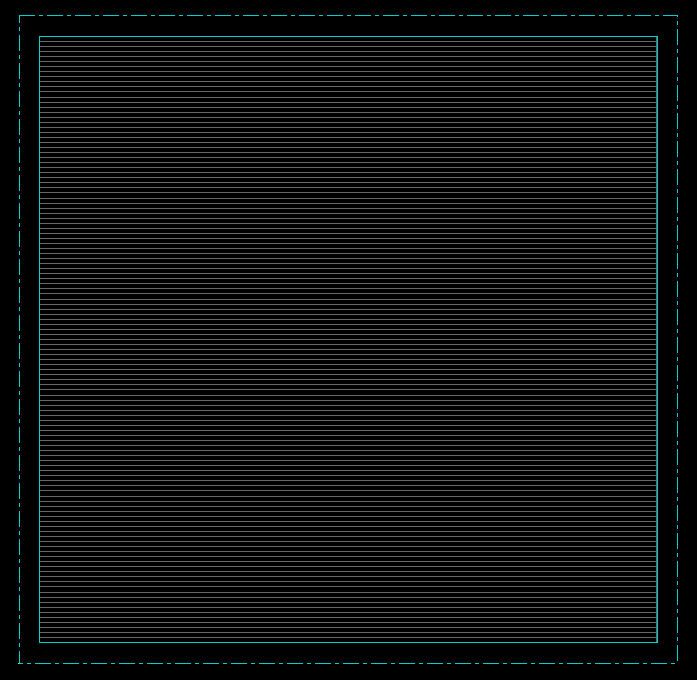
\includegraphics[scale=0.4]{pic/floorplan.png}
\end{center}


\subsection{PowerPlanning}
At this stage we connect the power nets that we had created in the design import step. We also added the power ring around the core and we specified the metal layer we wanted to use for the core ring as well as the width and spacing between them. We changed the “Top” and “Bottom” layers from M1 to M5, and “Left” and “Right” from M2 to M6. The top and bottom layers are noted H for Horizontal disposition and the others ones are noted V for Vertical disposition.\\

\begin{center}
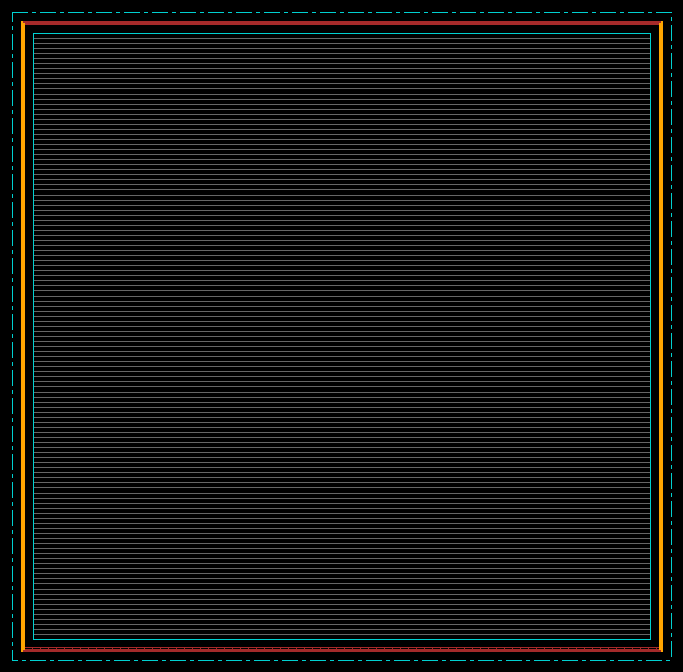
\includegraphics[scale=0.4]{pic/ring.png}
\end{center}
We use the M5 and M6 layers for power because these layers are bad timing perspective, and the power are static (0v/3.3V).\\
We also added the stripes to our design. We use the menu “Power > Power Planning > Add Stripes”. In the “Set Configuration” our power “vdd\_core gnd\_core” are printed besides the label “Net(s)”. For the “Layer” we have choose “M6” which is vertical and for the “Width” the same value as for the rings, 1.32, for the spacing we have choose 0.92. For the “Set-to-Set Distance” we put 50 in order to have a set of stripes every 30 microns. In the “Stripe Boundary” part we have leave “Core ring”. In the “First/Last Stripe” part we set to “Start From” “Left” and for the offset we put “X from left” to “25”.\\ 
We have checked that the stripes and the core ring where well connected.\\
\begin{center}
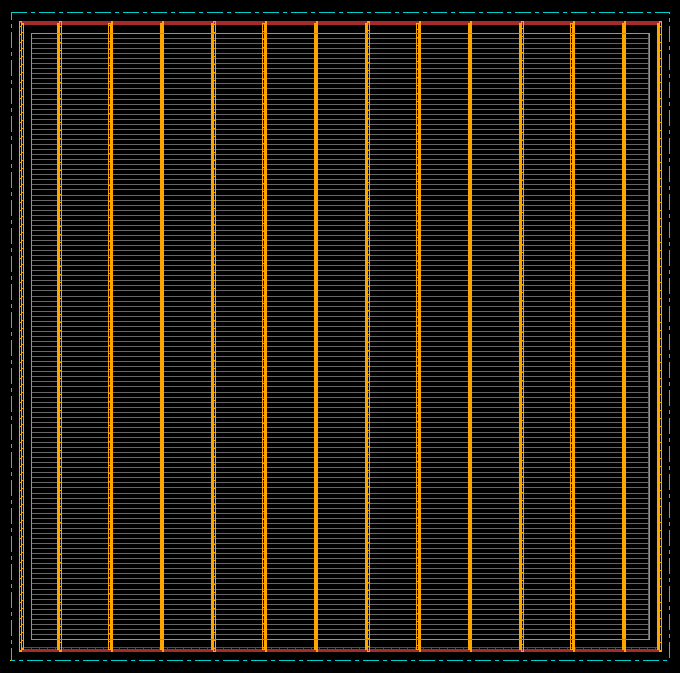
\includegraphics[scale=0.4]{pic/stripes.png}
\end{center}

For routing at this point we use the Special Router (SRoute) to route the “follow pins”. The follow pins are the horizontal stripes connecting all VDD and VSS metal chunks of the standard cells belonging to the same row. We used the “Route > Special Route” menu to connect the “vdd\_core” and “gnd\_core” to the standard cells pins. We specified to SRoute to not allow layer change and we checked the “follow pins” connections in our design.\\
\begin{center}
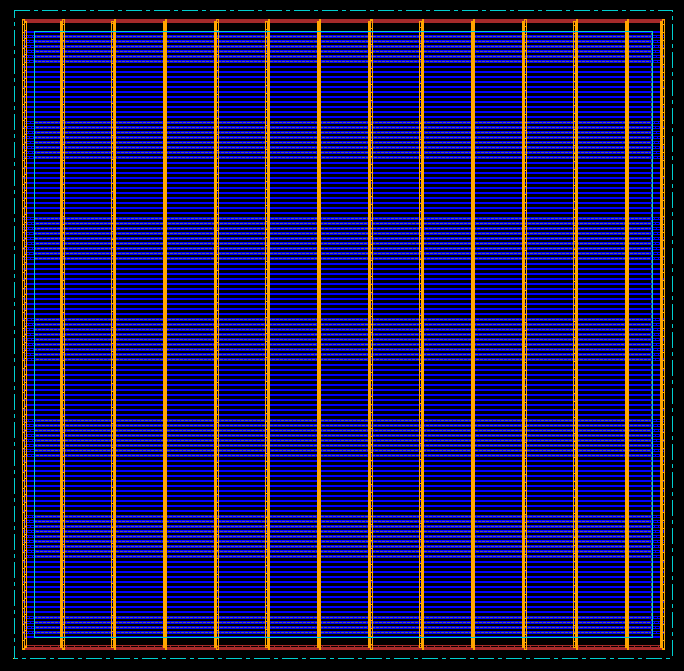
\includegraphics[scale=0.4]{pic/sroute.png}
\end{center}

Finally we checked our design with the command: “>checkDesign –floorplan”. After getting positive results we saved our floorplan in an “.fp” type of file.\\

\subsection{Place Design}
At this stage we place the standard cells of our design using the “Place > Standard Cells” menu. The result schematic design is shown in the figure:
\begin{center}
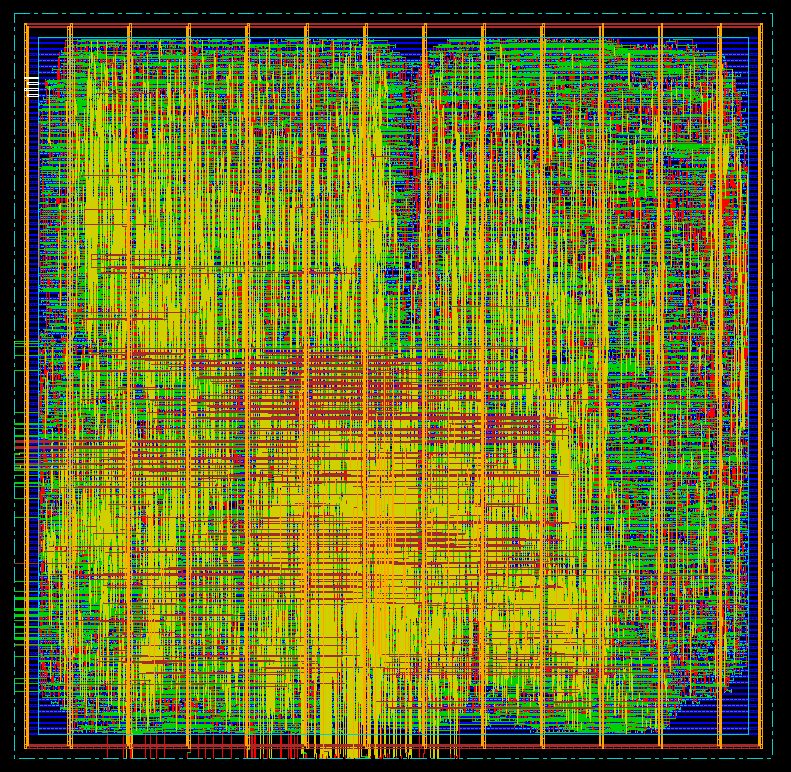
\includegraphics[scale=0.4]{pic/place.png}
\end{center}

\subsection{Trial Route}
In order to get a quick estimation of the route feasibility and timing, we use the “Route > Trial Route >prototyping” menu to perform a Trial Route. This tool runs a quick route without fixing DRC or LVS violations.

\subsection{Timing Analysis}
In order to verify that our timing constraints are met we performed a timing analysis starting with a RC extraction. After that, we use the “Timing > Analysis Condition > Specify Analysis Mode” menu in order to enable the setup analysis, we set the FE-DC as the delay calculator.  Finally using the “Timing > Analyze Timing” we performed the timing analysis menu. Given that we hadn’t done the Clock Tree Synthesis at this point, we set preCTS as “Design Stage”.\\

After performing the analysis we observed that our Worst Negative Slack (WNS) was negative, so we optimized our design using the “>optDesign preCTS” command. Then we check the new timing with the “> report\_timing” command. The results before and after optimization are shown in figure.\\

Is important to have the Total Negative Slack (TNS) information as wells as the WNS, because being the TNS the sum of all the paths that are violating our timing constraints, it gives us the level of slack severity of the whole design. So, If we have a high TNS, we should think in make some analysis and changes in our design and configurations, or decide whether to proceed or not with the current implementation.\\

\subsection{CTS}
\begin{center}
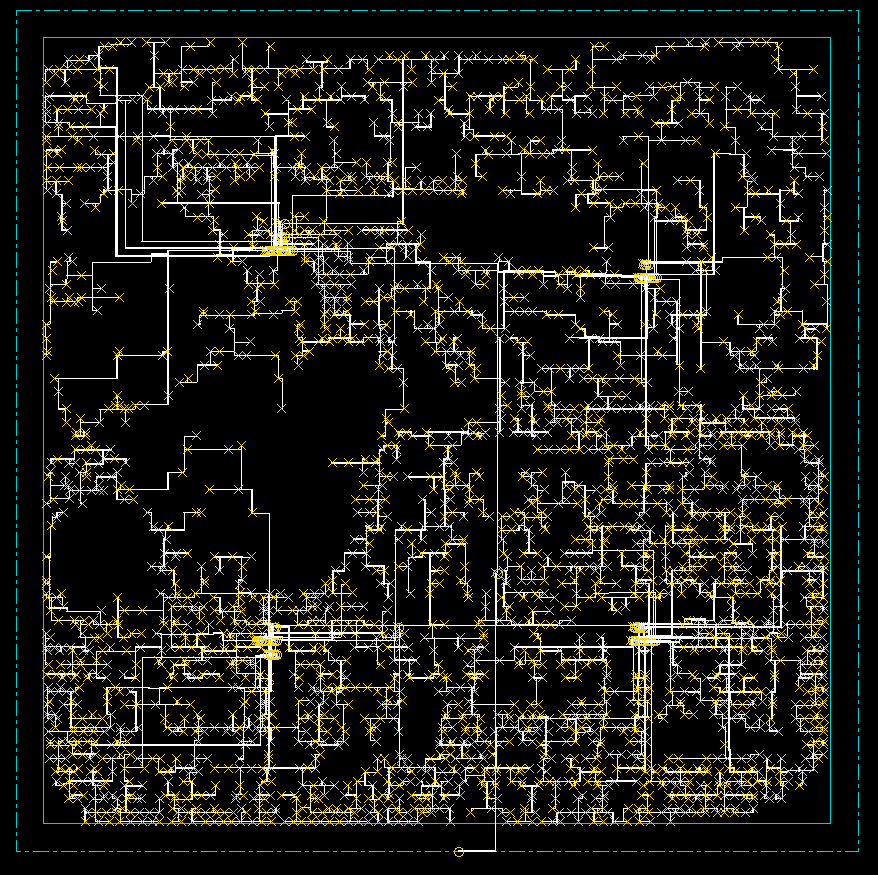
\includegraphics[scale=0.4]{pic/true/clock_tree.png}
\end{center}
\subsection{NanoRoute}
For routing our post CTS design we used NanoRoute module of SoC Encounter. After NanoRoute was finished, we perfomed a timing analysis using the “> timeDesign postRoute” command. We noted that our design didn’t met the timing constraints so we did some optimization using the “> optDesign postRoute”. The timing results before and after optimization are shown in figure:

\begin{center}
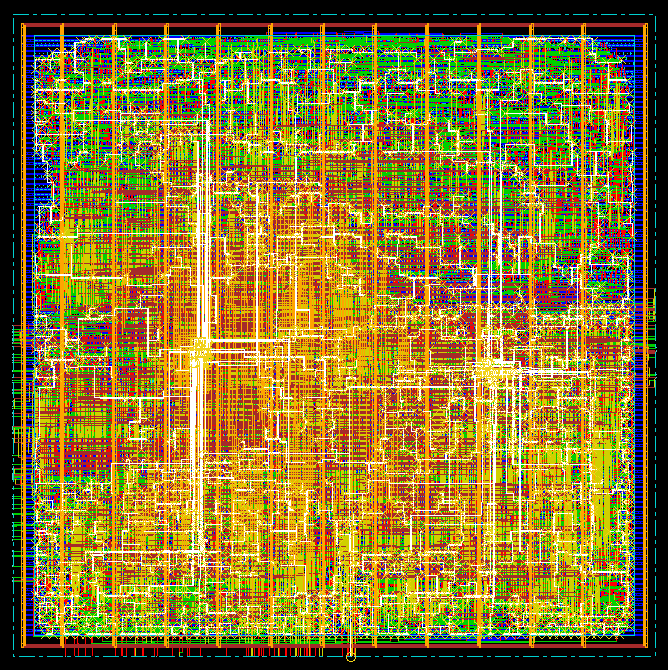
\includegraphics[scale=0.4]{pic/true/route_final.png}
\end{center}

\subsection{Adding filler cells}
After finishing the placing and routing phases in our circuit we proceeded to insert the filler cells using the “Place > Physical Cells > Add Filler” menu in SoC Encounter. We call it filler cells, because the fill the exiting space between the standard cells after the P \& R is done. Filler cells are primarily non-functional cells used to continue the VDD and VSS rails. They reduce the DRC Violations created by the base (NWell, PPlus \& NPlus) layers and help to maintain the Power Rail connection continuity.
\subsection{Verification}
Before we finish we also check the DRC, connectivity and the gemotry before generating the GDS file.
\end{document}
